
\chapter{Architecture du projet}

   
\section{Code fourni par le client}

Le code fourni par le client se compose de deux packages. 

\subsection{hl\_communication}

Le premier package \textbf{hl\_communication} contient les classes nécessaires à la lecture des messages des robots.
Nous avons d'une part de multiples fichiers .proto décrivant l'architecture des messages. Cette architecture est résumée dans le diagramme ci-dessous. Un message se compose de parties essentielles : les messages du Game\_Controller et ceux des robots.
\bigskip

\begin{figure}[h] 
\centering 
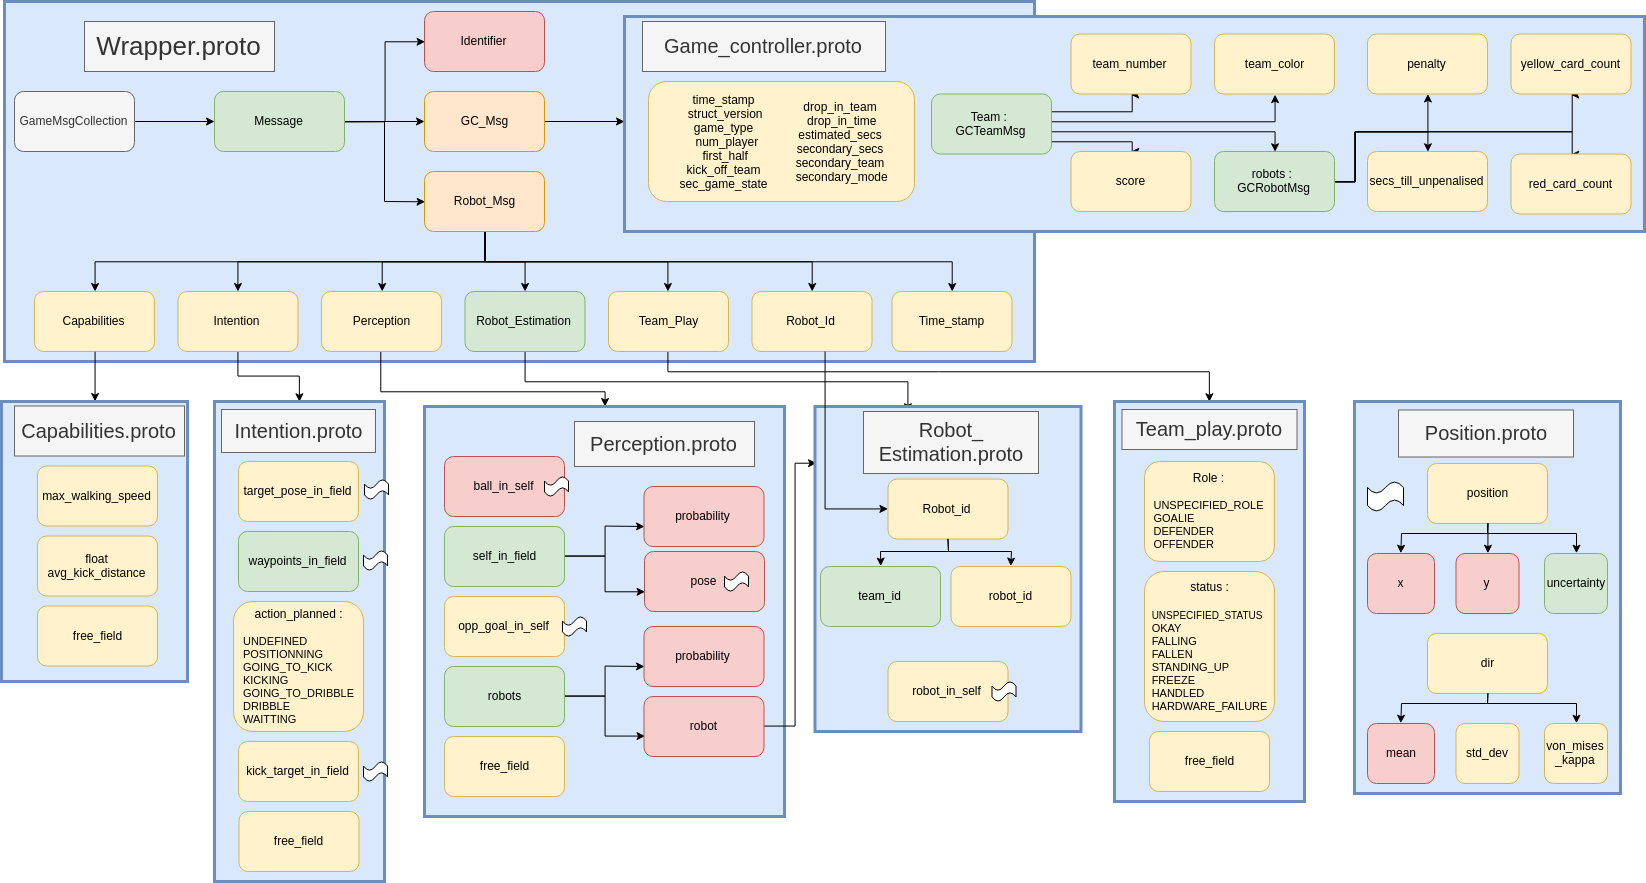
\includegraphics[scale = 0.22]{images/messages.png}
    \caption{Architecture des messages}
    \label{fig:message}
\end{figure} 


Le Game\_Controller GC\_Msg contient toutes les données réelles du match, c'est à dire toutes les données envoyées par la table d'arbitrage: le temps, les équipes (GCTeamMsg) et leurs robots (GCRobotMsg). 
\bigskip

Dans ces messages nous récupérons le numéro des équipes et le score.
On reçoit donc également un message Robot\_Msg par robot. Dans notre programme nous traitons plusieurs éléments de ces message :
\begin{itemize}
    \item le time\_stamp pour mesurer le temps écoulé depuis l'envoi du message.
    \item le Robot\_id : qui nous donne son numéro d'équipe et de robot.
    \item la Perception du robot : on récupère ici la position et la direction du robot (self\_in\_field) et de la balle (ball\_in\_self).
    \item Enfin, l'Intention du robot est utilisé pour avoir sa position souhaitée (target\_pose\_in\_field)
    
\end{itemize}
La position définie dans le fichier position.proto est réutilisée dans tous les éléments où l'on voit le "\textasciitilde". 
\bigskip

Les principales fonctions que l'on utilise de ce package sont contenues dans la classe MessageMonitoring dont nous utilisons principalement la fonction getStatus(time\_stamp) qui nous donne le message correspondant à un certains temps time\_stamp.
\bigskip

\subsection{hl\_monitoring}

Ce second package contient essentiellement le MonitoringManager qui nous permet de rythmer l'avancée de la vidéo. 
\bigskip

Tout d'abord, il lit le fichier de configuration match\_settings.json puis replay.json/live.json qui contient le nom du binaire où l'on récupère les messages des robots, les informations sur les caméras et leur vidéos et enfin un booléen pour savoir si on est en replay ou en live.

C'est également lui qui va initialiser le MessageManager vu précédemment. Tant que ce manager fonctionne, il va récupérer l'image à un temps donné de la vidéo. 
\bigskip

Il contient toutes les fonctions de calibration de la caméra notamment l'outil static\_calibration (qui nous permet de calibrer une caméra une fois que l'on a récupéré les paramètres intrinsèques) et la fonction fieldToImg qui transforme des positions du plan réel au plan de l'image en fonction des paramètres de la caméra. Enfin la dernière chose à noter et la classe Field qui permet d'afficher les lignes du terrain. 
\bigskip
\begin{figure}[h] 
\centering 
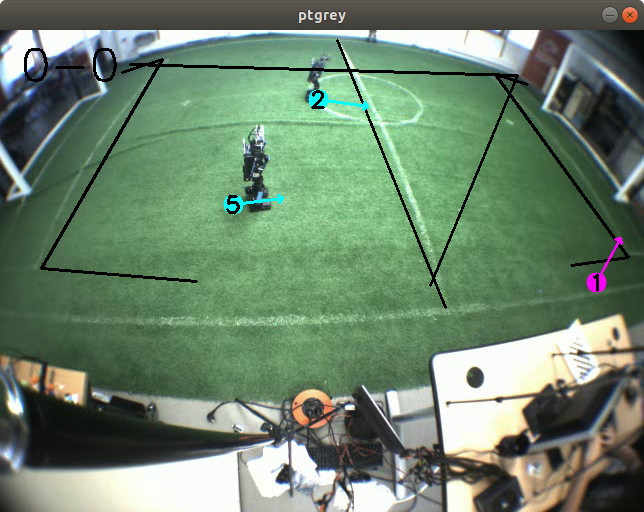
\includegraphics[scale = 0.3]{images/test2.png}
    \caption{Test sur l'affichage des lignes du terrain}
    \label{fig:field}
\end{figure} 


Elle nous permet de voir le bon fonctionnement ou non de la calibration de la caméra. Par exemple, la vidéo ptgrey.avi tournée le 20/02/2019, les lignes du terrains ne correspondent pas à la réalité. Nous pouvons voir sur la photo que la ligne de la zone du gardien proche du joueur 1 en rose est mal calibrée. Il faut noter en revanche que même si la ligne est mal placée, le robot est bien placé par rapport à la ligne.
\bigskip

Le package hl\_monitoring contient également basic\_monitoring un exécutable permettant de tester tout ce qui nous a été fourni par le client. C'est dans ce fichier que nous avions fait nos premiers tests d'affichage avant d'en recréer un nous-même.

\section{Architecture du code}

Nous avons ajoutés deux packages à ceux fournis par le client.

D'une part nous avons \textbf{Traitement} qui nous permet d'annoter la vidéo et de l'afficher d'une façon très basique et d'autre part \textbf{Interface} qui nous permet d'afficher la vidéo avec une interface utilisateur et de changer les annotations en cours de lecture.
\bigskip

Le Traitement se compose de différentes classes:
\begin{itemize}
    \item des classes outils telles que Position ou Direction : nous permettant de mieux gérer les éléments récupérés dans les logs. 
    \item les classes RobotInformation et Team : Team se compose d'une map de RobotInformation, elle est essentielle pour différencier les robots lors de la réception des messages. RobotInformation nous permet donc de stocker le dernier message de chaque robot et d'autres informations utiles aux annotations.
    \item la classe Annotation qui contient une fonction par annotation qu'il est possible d'ajouter.
\end{itemize}
\bigskip

Le fichier principal du traitement est test\_traitement, il permet de lancer la vidéo et d'annoter la vidéo grâce au deux fichiers de configuration match\_settings.json et annotation\_settings.json. Le détail des choix possibles pour ces fichiers se fera dans la partie suivant, fonctionnalités implémentées.
\bigskip

Enfin, nous pouvons retrouver trois fichiers de tests que l'on détaillera dans la partie appropriée.
\bigskip

/////////////////////////////////////
\bigskip
L'Interface a été conçue à partir de l'API Qt, [blabla parce que ... ??]. Elle est composé de différentes classes qui héritent de classes Qt :
\begin{itemize}
    \item MainWindow : hérite de QMainWindow, représente la fenêtre principal de l'interface.
    \item TeamPanel et RobotPanel : héritent de QWidget, ces deux classes nous permettent de faire savoir l'état d'une annotation pour chaque robot via des QLabel.  
    \item ChoiceDialog : hérite de QDialog, représente la fenêtre pop-up servant à modifier les choix d'Annotation.
    \item ChoiceComboBox : hérite de QWidget, permet de sélectionner le numéro d'une équipe et d'un robot. Crée par choix de factorisation puisque ce mode de choix était présent 3 fois dans ChoiceDialog.
\end{itemize}
\bigskip

Le fichier principal main permet d'exécuter l'interface.
\bigskip

Voici donc comment se trouve notre architeture :

\begin{figure}[h] 
\centering 
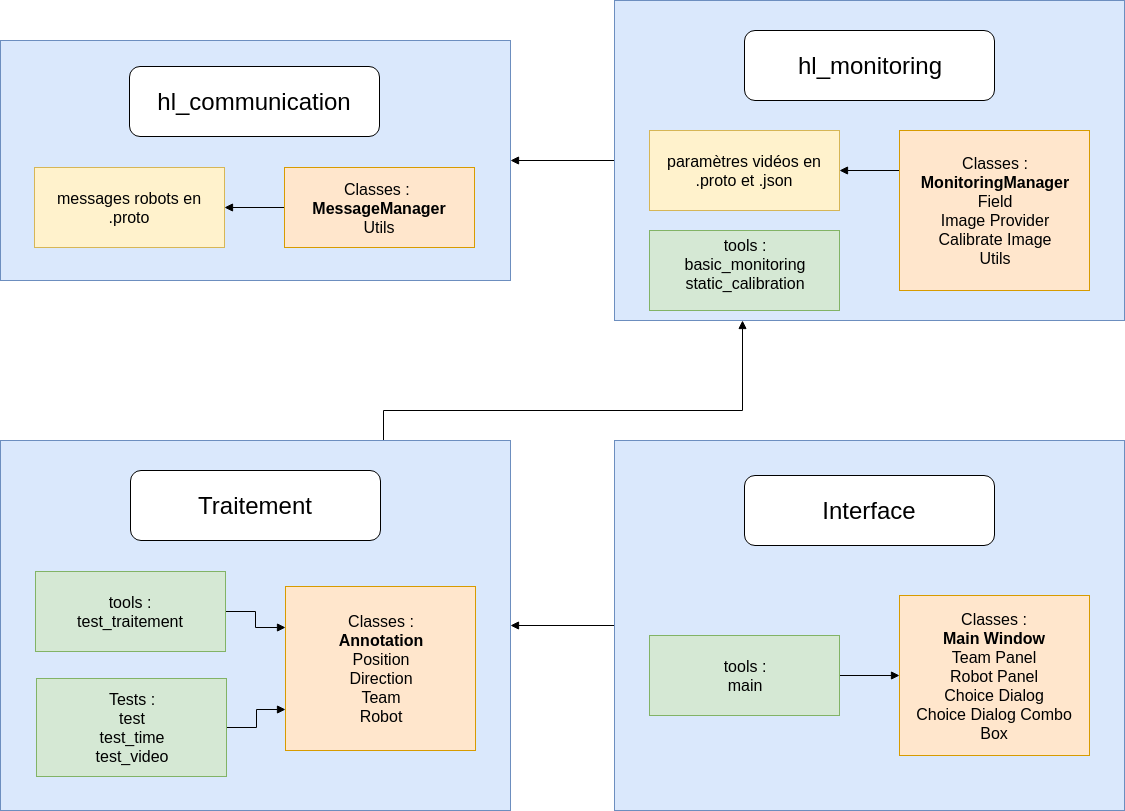
\includegraphics[scale = 0.3]{images/archiprojet.png}
    \caption{Architecture des packages}
\end{figure} 


\section{Différence v1}


On verra si on a pas la flemme

Lors de notre rendu de la V1 en début d'année, notre architecture n'était pas adaptée


\section{Fonctionnement du projet}

Pour expliquer le fonctionnement de notre projet, nous allons nous appuyer sur le Traitement essentiellement, sachant que l'interface fonctionne de la même façon avec les outils d'affichage en plus.

\subsection{L'initialisation}

Au lancement de l'exécutable du traitement, main\_traitement, deux fichiers sont indispensables comme nous pouvons le voir dans la Figure~\ref{fig:archi} ci\_dessous. 


\begin{figure}[H] 
\centering 
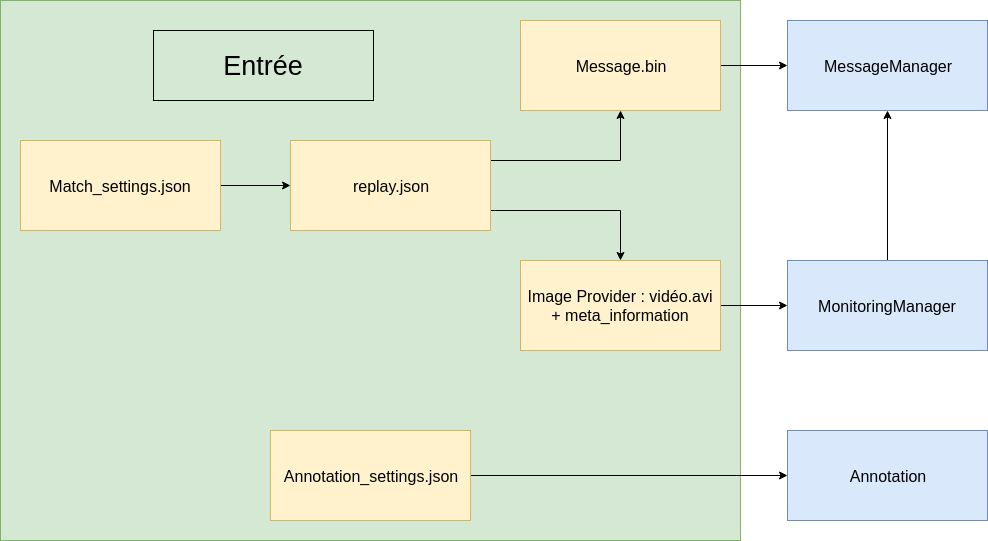
\includegraphics[scale = 0.3]{images/init.png}
    \caption{Architecture des packages}
    \label{fig:archi}
\end{figure} 
\bigskip


Le premier, match\_settings contient la configuration du projet qui va être dans un fichier replay.json ou live.json.
Le fichier replay.json contient d'une part le nom du binaire contenant les messages permettant de créer un MessageManager et d'autre part le nom de la vidéo à traiter ainsi que du binaire contenant les informations de la caméra associée permettant d'avoir le MonitoringManager.
\bigskip

Malheureusement, nous n'avons pas pu tester notre programme en live donc nous n'allons pas détailler les informations du live.json.
\bigskip

Le second fichier indispensable est annotation\_settings.json qui nous permet de créer un objet Annotation qui lit le fichier et prend en compte tous les paramètres nécessaires à chaque annotation.

À l'initialisation, nous créons également la variable "now" qui est un time\_stamp et qui rythme l'avancée de la vidéo.

\subsection{La récupération d'un message}

Avant de nous occuper des images des vidéos, nous récupérons le message associé au time\_stamp. 

Comme nous pouvons le voir dans la Figure~\ref{fig:log}, nous récupérons d'une part les informations de chaque Team (le score) et des RobotInformation (le Robot\_Msg). Nous accédons au robot à travers leur Team.
\begin{figure}[h] 
\centering 
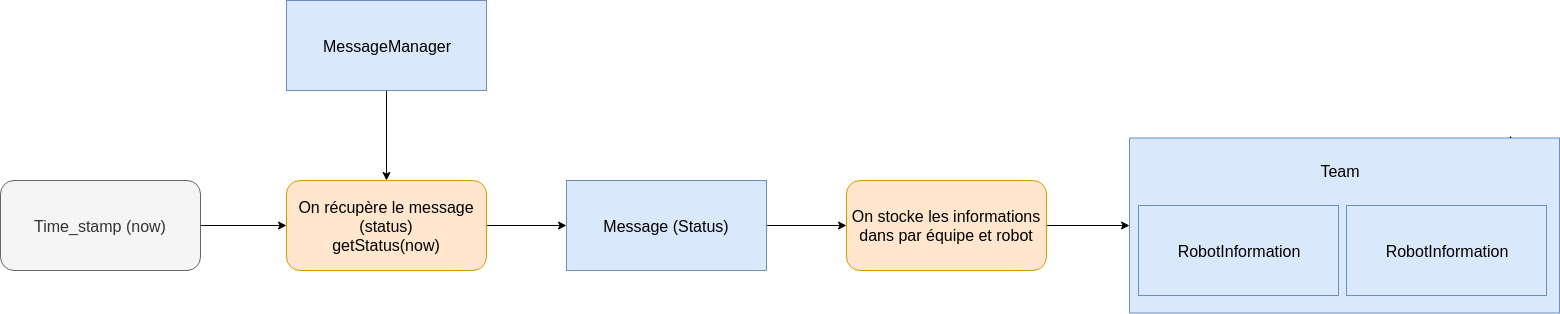
\includegraphics[scale = 0.24]{images/logs.png}
    \caption{Récupération des messages}
    \label{fig:log}
\end{figure} 


\subsection{La récupération d'une image}

À chaque time\_stamp, nous allons donc récupérer l'image associé mais il est possible de lancer plusieurs vidéos en simultané. La récupération d'une image se fait donc comme détaillée Figure~\ref{fig:img} : 

\begin{figure}[h] 
\centering 
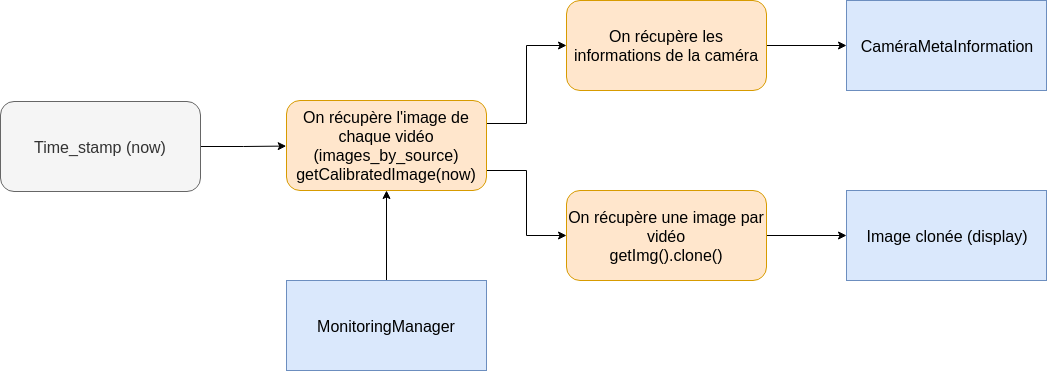
\includegraphics[scale = 0.3]{images/image.png}
    \caption{Récupération des images}
    \label{fig:img}
\end{figure} 

Nous récupérons d'abord une map avec une image par vidéo puis nous récupérons une image et les meta-informations de la caméra associé. L'affichage se fait donc image par image pour chaque vidéo, c'est ce qui permet d'afficher deux vidéos en simultané.

\subsection{L'annotation sur l'image}

Maintenant que nous avons récupéré tous les éléments, nous pouvons annoter l'image comme on le voit Figure~\ref{fig:annot}. Nous affichons image par image et robot par robot. Le time\_stamp nous permet de savoir si le dernier message du robot n'est pas trop vieux et à définir l'opacité pour l'affichage optimisé.

\begin{figure}[h] 
\centering 
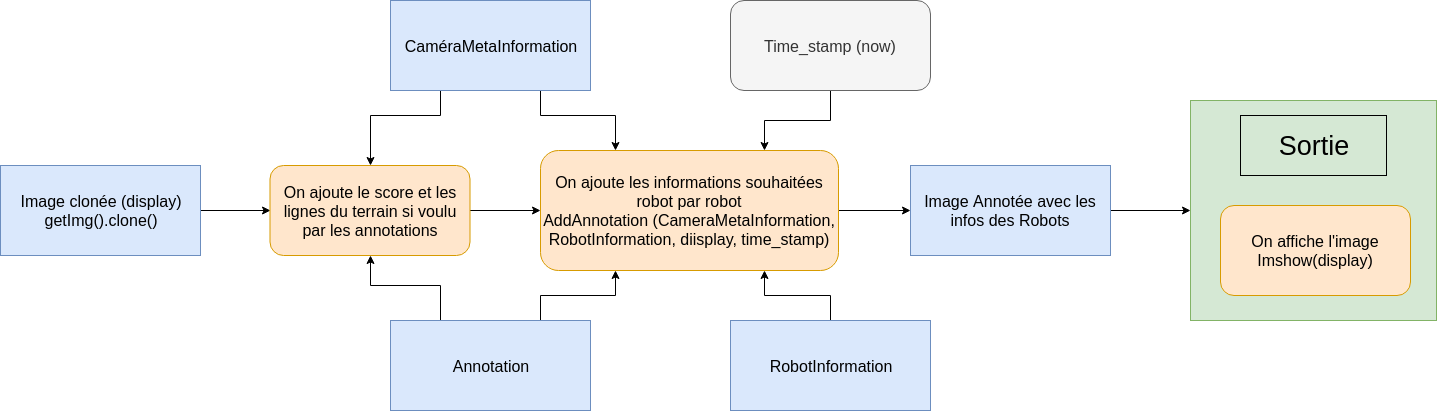
\includegraphics[scale = 0.27]{images/annotation.png}
    \caption{Annotation des images}
    \label{fig:annot}
\end{figure} 

Notre classe d'annotation comprend la fonction AddAnnotation globale et une fonction par annotation (par exemple : annotePosition, annoteDirection ..).
\bigskip


Dans la fonction AddAnnotation, nous décomposons le message contenu par le RobotInformation.


Si les éléments que nous souhaitons annoter sont présents alors nous regardons si l'utilisateur veut afficher l'annotation.


Si les deux conditions sont remplies, alors nous appelons la fonction de l'annotation adéquate. 
